%\documentclass[<options>]{elsarticle}
\documentclass [sort&compress] {elsarticle}
\usepackage{graphicx}% Include figure files

\bibliographystyle{elsarticle-num}
\begin{document}
\begin{frontmatter}

\title{Influence of $\gamma$--irradiation and ultrasound treatment on carrier transport in Au�-SiO$_2$�-Si structure}

\author{A.M.~Gorb}
\author{O.A.~Korotchenkov}

\author{O.Ya.~Olikh\corref{cor1}}
\ead{olikh@univ.kiev.ua}

\author{A.O.~Podolian}
\author{R.G.~Chupryna}

\cortext[cor1]{Corresponding author}



\address{Faculty of Physics, Taras Shevchenko National University of Kyiv, Kyiv 01601, Ukraine}


\begin{abstract}
The effect of  $^{60}$Co $\gamma$--irradiation ($5\cdot10^7$~rad) and ultrasound treatment (4~MHz, 2~W/cm$^2$, up to 60 min) on current--voltage characteristics is experimentally investigated for Au�-SiO$_2$�-Si structure.
The modification of carrier transport  as well as defect subsystem is analysed.
In particular,  it is shown that irradiation causes the space charge limited current and the trap--assisted tunneling current.
Experimental observations of the acoustically induced nearly room--temperature annealing of
$P_b$-- and $E'$---centres and partial recovering of irradiated silicon MOS structure characteristics are highlighted.
\end{abstract}




\begin{keyword}
MOS structures\sep Si�-SiO$_2$ interface\sep ultrasound treatment\sep $\gamma-$rays
\end{keyword}


\end{frontmatter}


\section{Introduction}


It is well known that the defects are crucial for the semiconductor devices performance.
Thus electrical characteristics of metal--oxide--semiconductor (MOS) structure are  extremely sensitive to the interface state density.
The formation of lattice defects near the interface caused by the irradiation is very harmful for such device performance and leads to the current mechanism change frequently \cite{Rao,Tascioglu2010old,Tataroglu:2007NIMA,Olikh:2013IEEE,Verma,Abdolahpour}.
The radiation defects (RDs) are known to be able to effectively interact with elastic acoustic vibrations.
E.g. the RDs are annealed by acoustic waves treatment at temperature, which is much lower than ones in the case of ultrasound-free heating.
Such phenomenon is observed in the single crystal of Si \cite{Podolian2012, PodolHivrEn, YOlikh2006TPL}, Ge \cite{Olikh:FTP1996} as well as  semiconductor \cite{OlikhProc, OstrovFTTRad} and alkaline halide \cite{UST:OstrovCsI} compounds.
Usually it deals with a decay of radiation--formed complexes and acoustically induced (AI) diffusion of defects to a sink.
Besides, the possibility of parameter recovery of irradiated barrier structures by ultrasound treatment (UST) is shown.
So, the active ultrasound effects are observed in the solar cells \cite{YOlikh2007TPL,Olikh2018JAP}, LEDs \cite{US:LED,UST:LED_SM}, and Schottky diodes \cite{Pashaev2014,Olikh:Ultras}.
The   industrially important Si--SiO$_2$ system is under consideration as well.
Particularly, the AI change of the Si--SiO$_2$ interface defects \cite{Ostap:SiO2,UST:Medvid,Zaver:2008}
and minority carrier lifetime \cite{Parchinskii2003,Zdeb1989,Gorb2010} are reported.

Some attention is paid to the UST of silicon MOS structures, which have been irradiated by $^{60}$Co $\gamma$--rays \cite{Parchinskii2000,Parchinskii2006}.
%The structures Si--SiO$_2$, produced by thermal oxidation of silicon with the specific resistance $0.2$~$\Omega\cdot$cm, have been under consideration.
The decrease of the both radiation--induced charge in the dielectric layer and  generation lifetime in the silicon,  and the insignificant growth of the surface recombination rate
after UST have been determined by capacitance�voltage characteristics measurements \cite{Parchinskii2000,Parchinskii2006}.

The first aim of our work is to investigate experimentally the UST influence on a charge transfer in the irradiated Au--SiO$_2$--Si structures.
In contrast to the cited study \cite{Parchinskii2000,Parchinskii2006},
our results are obtained
i)~for systems with a significantly higher RD concentration (see Section~\ref{Exp});
ii)~for operating mode of diode, that is, when the current was present.
It should be noted that our some result was reported previously \cite{Gorb2010}.
But this work is focused on the modification  of charge transfer mechanisms as well as the defect structure due to irradiation and UST.

On the other hand, in the silicon solar cell industry, the efficiency of a cell is restricted
by the recombination of carriers \cite{COLLETT201750}.
The silicon surface is often highly recombination active due to the abundance of band--gap states that exist due to dangling bonds.
The number of band--gap states can be reduced by introducing a dielectric coating.
The alneal is one of the most effective methods of passivating the Si--SiO$_2$ interface \cite{COLLETT201750,Kerr_2001,Aberle2000}.
This reaction is reported to release atomic hydrogen that is then free to diffuse across the oxide and passivate dangling bonds at the oxide--silicon interface \cite{Kerr_2001,Aberle2000,Larionova2010}.
In this work, it is demonstrated that it is possible to enhance the hydrogen diffusion by ultrasound.
Therefore, acousto--alneal can be effective processing step.



\section{Experimental and calculation details}
\label{Exp}

Experiments were performed on $n$-type (111)--oriented crystalline float-zone Si with residual boron (B) impurity concentration of about $10^{12}$~cm$^{-3}$ and doping phosphorus (P)
impurity concentration of $2\cdot10^{12}$~cm$^{-3}$.
The corresponding resistivity is $4000$~$\Omega\cdot$cm.
A bulk silicon material was divided into several rectangular--shaped samples of approximately
$1\times5\times10$~mm$^3$.
The MOS structures were formed by chemical etching of the upper Si surfaces using
HF-HNO$_3$--CH$_3$COOH solutions (HF:HNO$_3$:CH$_3$COOH~$=3:5:3$), followed by the surface oxidation due to the exposure to ambient air for 24 hours and the Au vacuum evaporation.
GaZn--eutectic Ohmic contacts were rubbed on the bottom surfaces of the samples.

The samples were $\gamma$--irradiated ($^{60}$Co source) at nominal room temperature to the dose $5\cdot10^7$~rad.
The measurement on the reference bulk sample shown that the conductivity has been reduced to about 0.5 of the initial value after irradiation.
As it was mentioned above, the ultrasonical recovering of the $\gamma$--irradiated silicon MOS structures  has been investigated \cite{Parchinskii2000,Parchinskii2006} early.
The structures Si--SiO$_2$, which have been produced by thermal oxidation of silicon, were under consideration \cite{Parchinskii2000,Parchinskii2006} as well.
But the more heavy degradation and the higher RD concentration were expected in the our case.
The main reasons are following.
i)~The high doze was used ($5\cdot10^7$~rad in our case as against $10^6$~rad in \cite{Parchinskii2000,Parchinskii2006} case).
ii)~The semiconductor resistivity was greater ($4000$~$\Omega\cdot$cm as against $0.2-0.5$~$\Omega\cdot$cm);
therefore  the non--ionizing energy losses was larger as well.
iii)~It is known \cite{PersenkovBook}, that the surface defect density, which is $\gamma$--induced in Si--SiO$_2$,  is about $10^{12}$~eV/cm for  $10^{7}$~rad in the case of (111)--oriented substrate and this value is much more then one for (100)--substrate, which is used in cited study.

The UST of the irradiated structure was done by attaching the piezoelectric transducer to one side of the sample. An epoxy glue was used as the bondingmedium, providing the rigid coupling of the transducer to the sample. The thickness resonant of the transducers was 4~MHz. A radio--frequency voltage supplied from a generator drives the transducer, resulting in vibrations of the coupled transducer-sample system.
UST was carried out by a two consecutive loading--unloading cycles, 30~min each;
so the total UST time $t_\mathrm{UST}$ was equal to 30~min or 60~min.
The density of acoustic energy flux $W_{US}$ in Si was equal to about 2~W/cm$^2$.
The sample temperature was measured with a copper--constantan thermocouple directly attached to the surface and did not exceed 350~K.
The more details about the sample and UST setup are presented elsewhere \cite{Gorb2010}.

The characteristics of the Au�-SiO$_2$�-Si structure, after $\gamma$--irradiation and after UST, were investigated using an  current--voltage ($I-V$) technique.
The forward and reverse bias characteristics were measured in current range from $10^{-9}$ to $10^{-3}$~A with a voltage step of 0.01 V at 295~K.

The data non--linear fitting were done by using the method of modified artificial bee colony \cite{MABC}.

\section{Results and Discussion}

Fig.~\ref{figIV} shows $I�V$ characteristics for both initial and irradiated Au--SiO$_2$--Si structure as well as after the sequent USTs.
One can see that $I�V$ characteristic for non-irradiated sample is typical for Schottky  diode:
the forward current is caused by a  thermionic emission (TE) over barrier,
the reverse current value is determined by  barrier height lowering, which occur due to the electric field ($\log I\sim V^{1/2}$) \cite{Rhoderick1988,Andrews}.
The forward branch was fitted by the following equation
\cite{Rhoderick1988}
\begin{equation}
\label{eqSDIV}
I=I_s\left\{\exp\left[\frac{q(V-IR_s)}{nkT}\right]-1\right\}\,,
\end{equation}
where
$I_s$ is the saturation current,
$R_s$ is the series resistance,
$n$ is the ideality factor,
the other symbols  have their usual meanings.
The fitting results are shown on Fig.~\ref{figIV}(b) and (d) by solid lines,
the obtained parameters values are listed in Table~\ref{tabMIS}.
It should be noted that the oxide layer presence does not allow to determinate the barrier height by help the saturation current value only,
%and equation $I_s=AA^*\,T^2\exp\left(-\frac{q\Phi_b}{kT}\right)$
%($A$ is the structure area,
%$A^*$ is the effective Richardson constant),
since the tunneling must be taken into account as well \cite{OZBEK2011,Kobayashi}.


\begin{figure}
\centerline{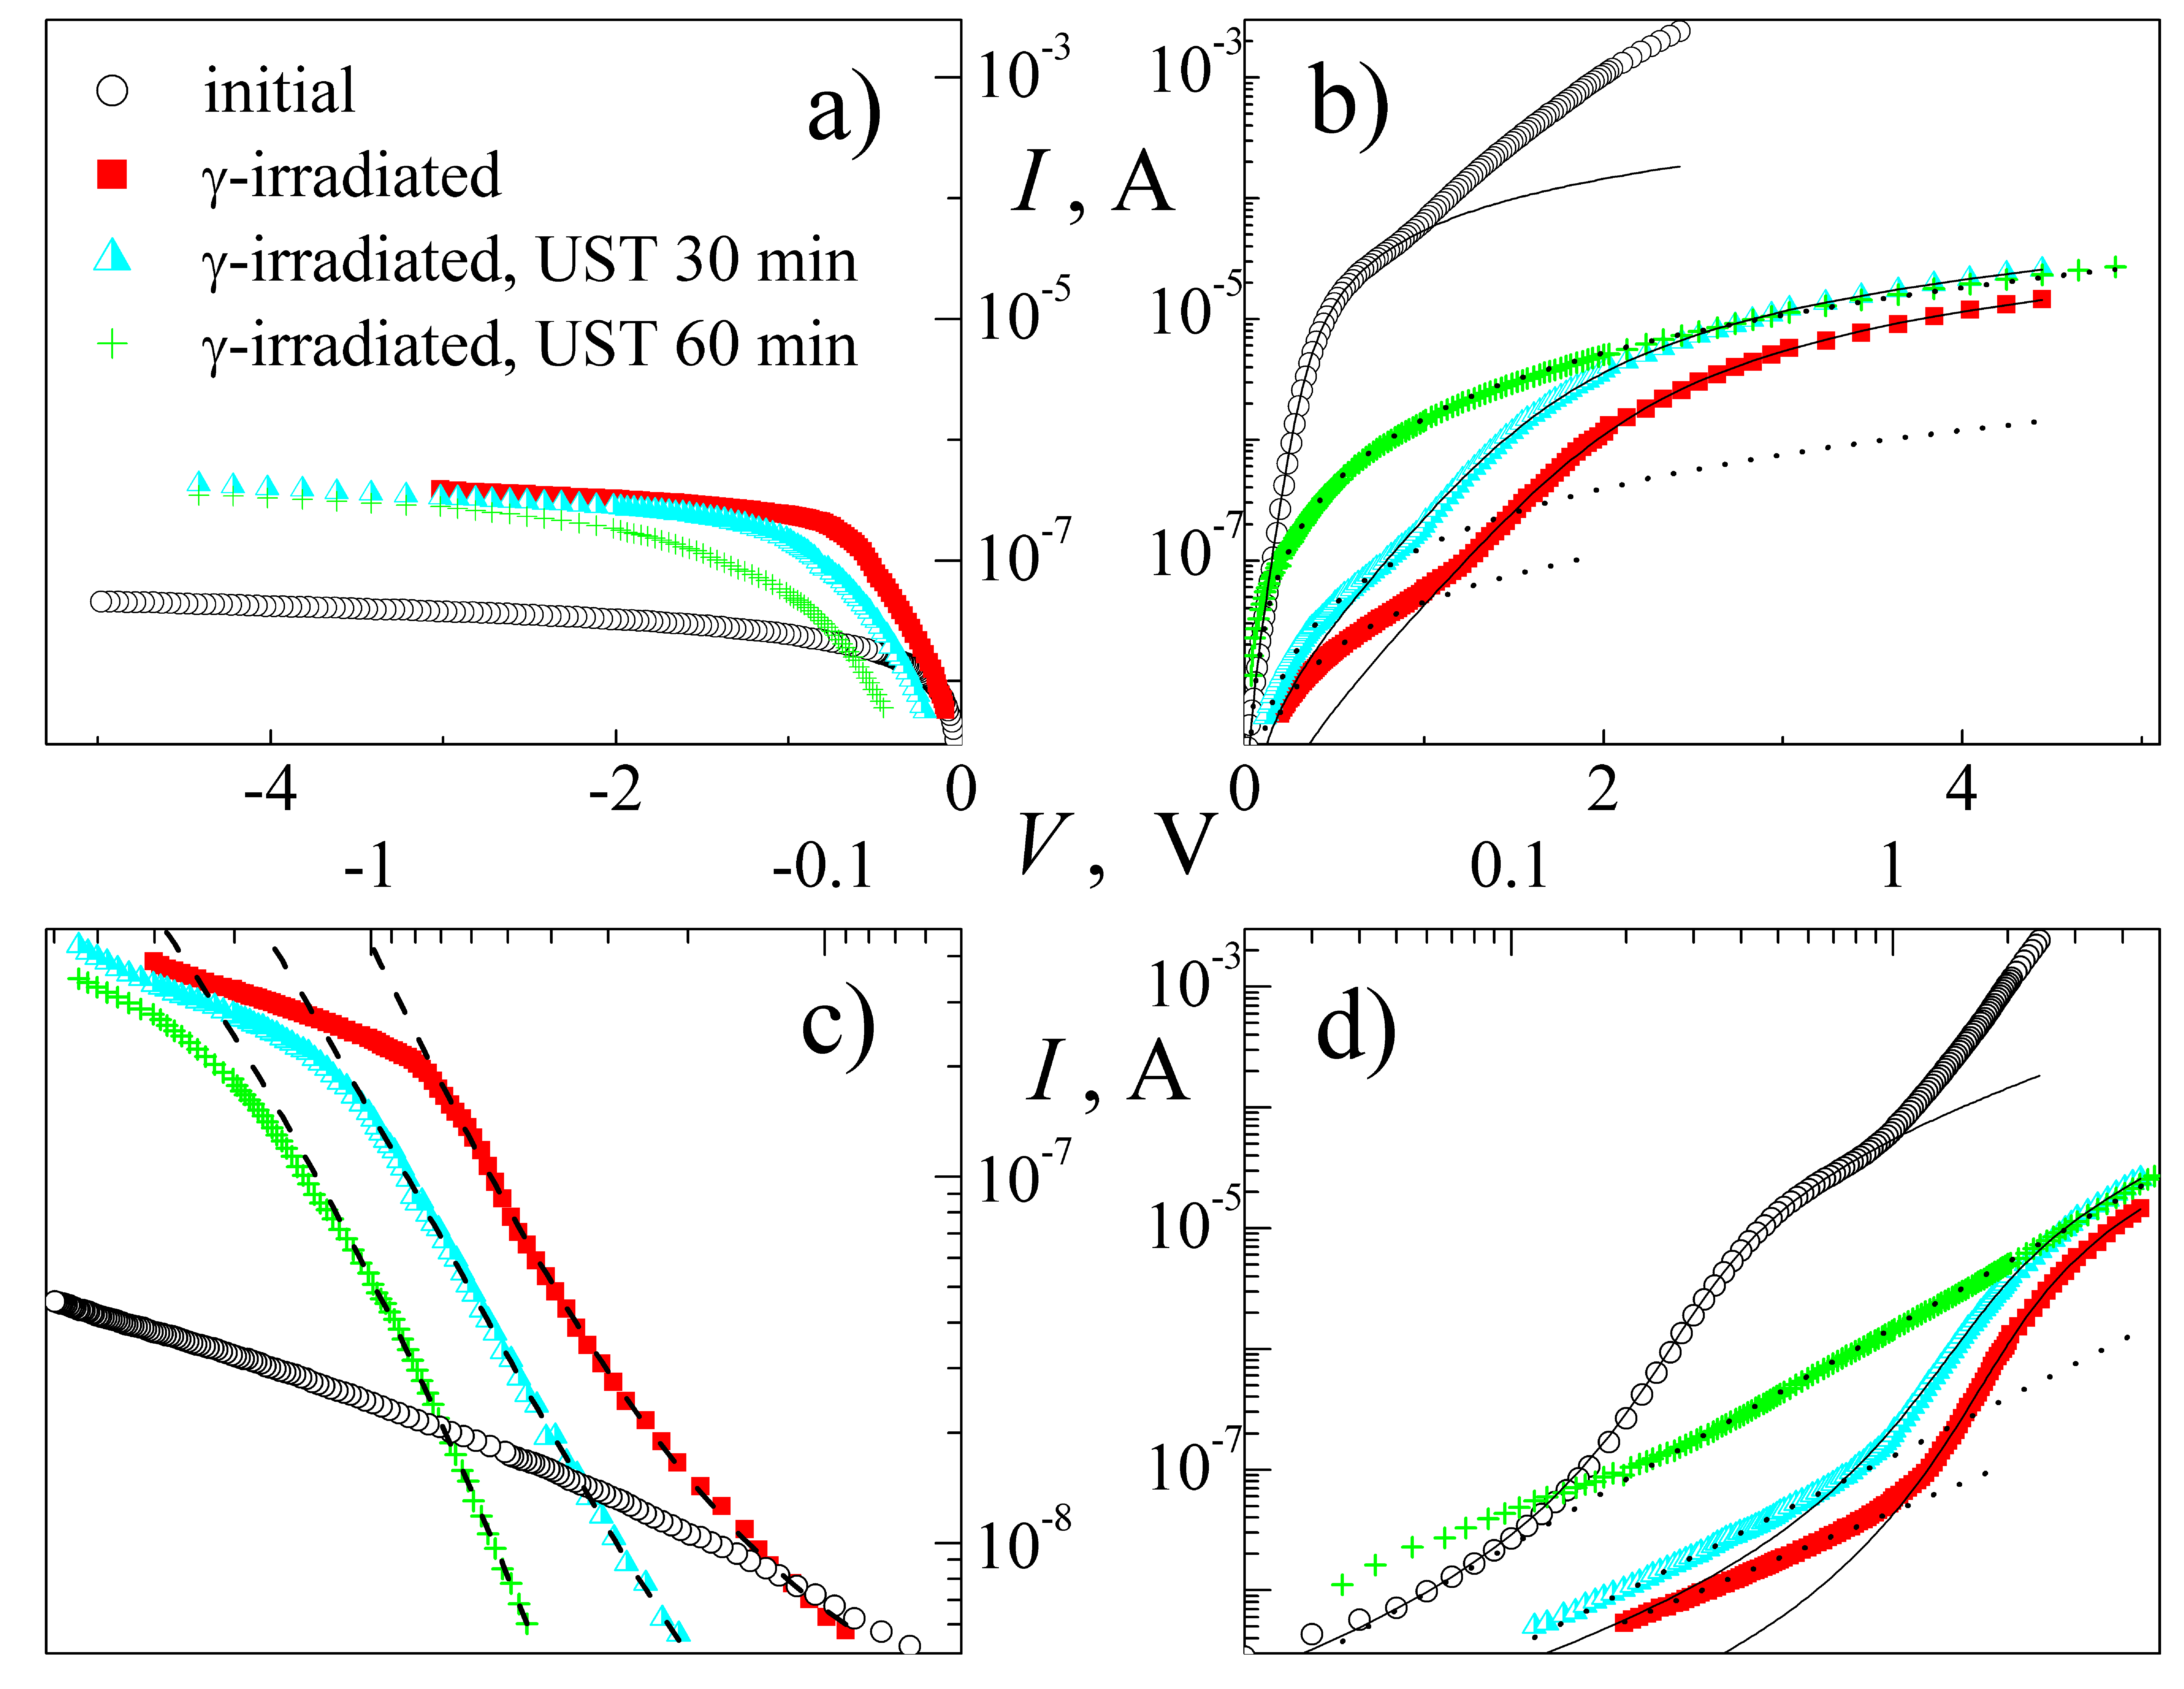
\includegraphics[width=0.95\textwidth]{figIV}}
\caption{\label{figIV}
The logarithmical (a, b) and double-logarithmical (c, d) plots of the reverse (a, c) and forward $I-V$ characteristics for Au--SiO$_2$--Si structure before and after $\gamma$--irradiation and UST.
$T=300$~K.
The marks are the experimental results,
and the solid, dashed, and dotted lines are the TE, TAT, and SCLC fitted curves using Eq.~(\ref{eqSDIV}), (\ref{eqIVTAT}), and (\ref{eqVIsclc}) correspondingly.
}%
\end{figure}




\begin{table}
\caption{\label{tabMIS}Extracted parameters for the Au--SiO$_2$--Si structure
}
\center
\begin{tabular}{lcccc}
\hline
\multicolumn{5}{l}{Structure status}\\\hline
$\gamma$--irradiation&$-$&$+$&$+$&$+$\\
UST&$-$&$-$&$+$&$+$\\
$t_\mathrm{UST}$ (min)&$0$&$0$&30&60\\ \hline
\multicolumn{5}{l}{Parameter}\\\hline
$I_s$ ($10^{-9}$A) & $3.3\pm0.3$& $1.1\pm0.2$& $4.9\pm0.5$&$-$ \\
$R_s$ ($10^{4}$��) & $1.1\pm0.2$& $13\pm1$& $9\pm1$&$-$ \\
$n$ & $1.7\pm0.1$& $10.3\pm0.2$& $9.9\pm0.2$& \\
$m_\mathrm{F}$ &$-$ &$1.30\pm0.05$& $1.6\pm0.05$& $1.8\pm0.05$ \\
$I_0$ ($10^{-8}$A) &$-$ &$5\pm1$& $13\pm2$& $150\pm10$ \\
$I_{0,\mathrm{TAT}}$ (a.u.) &$-$ &1& $0.14\pm0.03$& $0.04\pm0.01$ \\
$U_d$ (V) &$-$ &$0.7\pm0.1$& $0.44\pm0.05$& $0.12\pm0.05$ \\
$R_\mathrm{TAT}$ (a.u.) & &1& $0.54\pm0.05$& $0.33\pm0.04$ \\
$K_{\mathrm{RECT},\,\,0.5\mathrm{V}}$ &$800\pm100$ &$0.22\pm0.03$& $1.3\pm0.2$& $5.4\pm0.8$ \\
\end{tabular}
\end{table}


In addition, the real current value for the non-irradiated structure exceeds one, which is expected from Eq.~(\ref{eqSDIV}) --- see Fig.~\ref{figIV}.
The redundant current is most likely to be caused by the tunneling through the SiO$_2$ layer and can be described as \cite{Rhoderick1988,Novikov2009}:
\begin{equation}\label{eqFowlNord}
    \ln\left(\frac{I}{F_m^2}\right)\propto -\frac{4 \sqrt{2m^*}(qE_{\mathrm{eff}})^{3/2}}{3\hbar q F_m}\,,
\end{equation}
where
$F_m$ is the electric field,
$E_{\mathrm{eff}}$ is the effective tunneling energy.
%This assumption benefit is the linearity of the Fowler--Nordheim plots of the forward current at large bias --- see Fig.~\ref{FigFauler}.
The linearity of the Fowler--Nordheim plot of the forward current at large bias is this assumption evidence --- see Fig.~\ref{FigFauler}.
It was taken into account when plotting that the electric field in a oxide layer is proportional to the applied voltage $F_m\propto V$.

\begin{figure}
\centerline{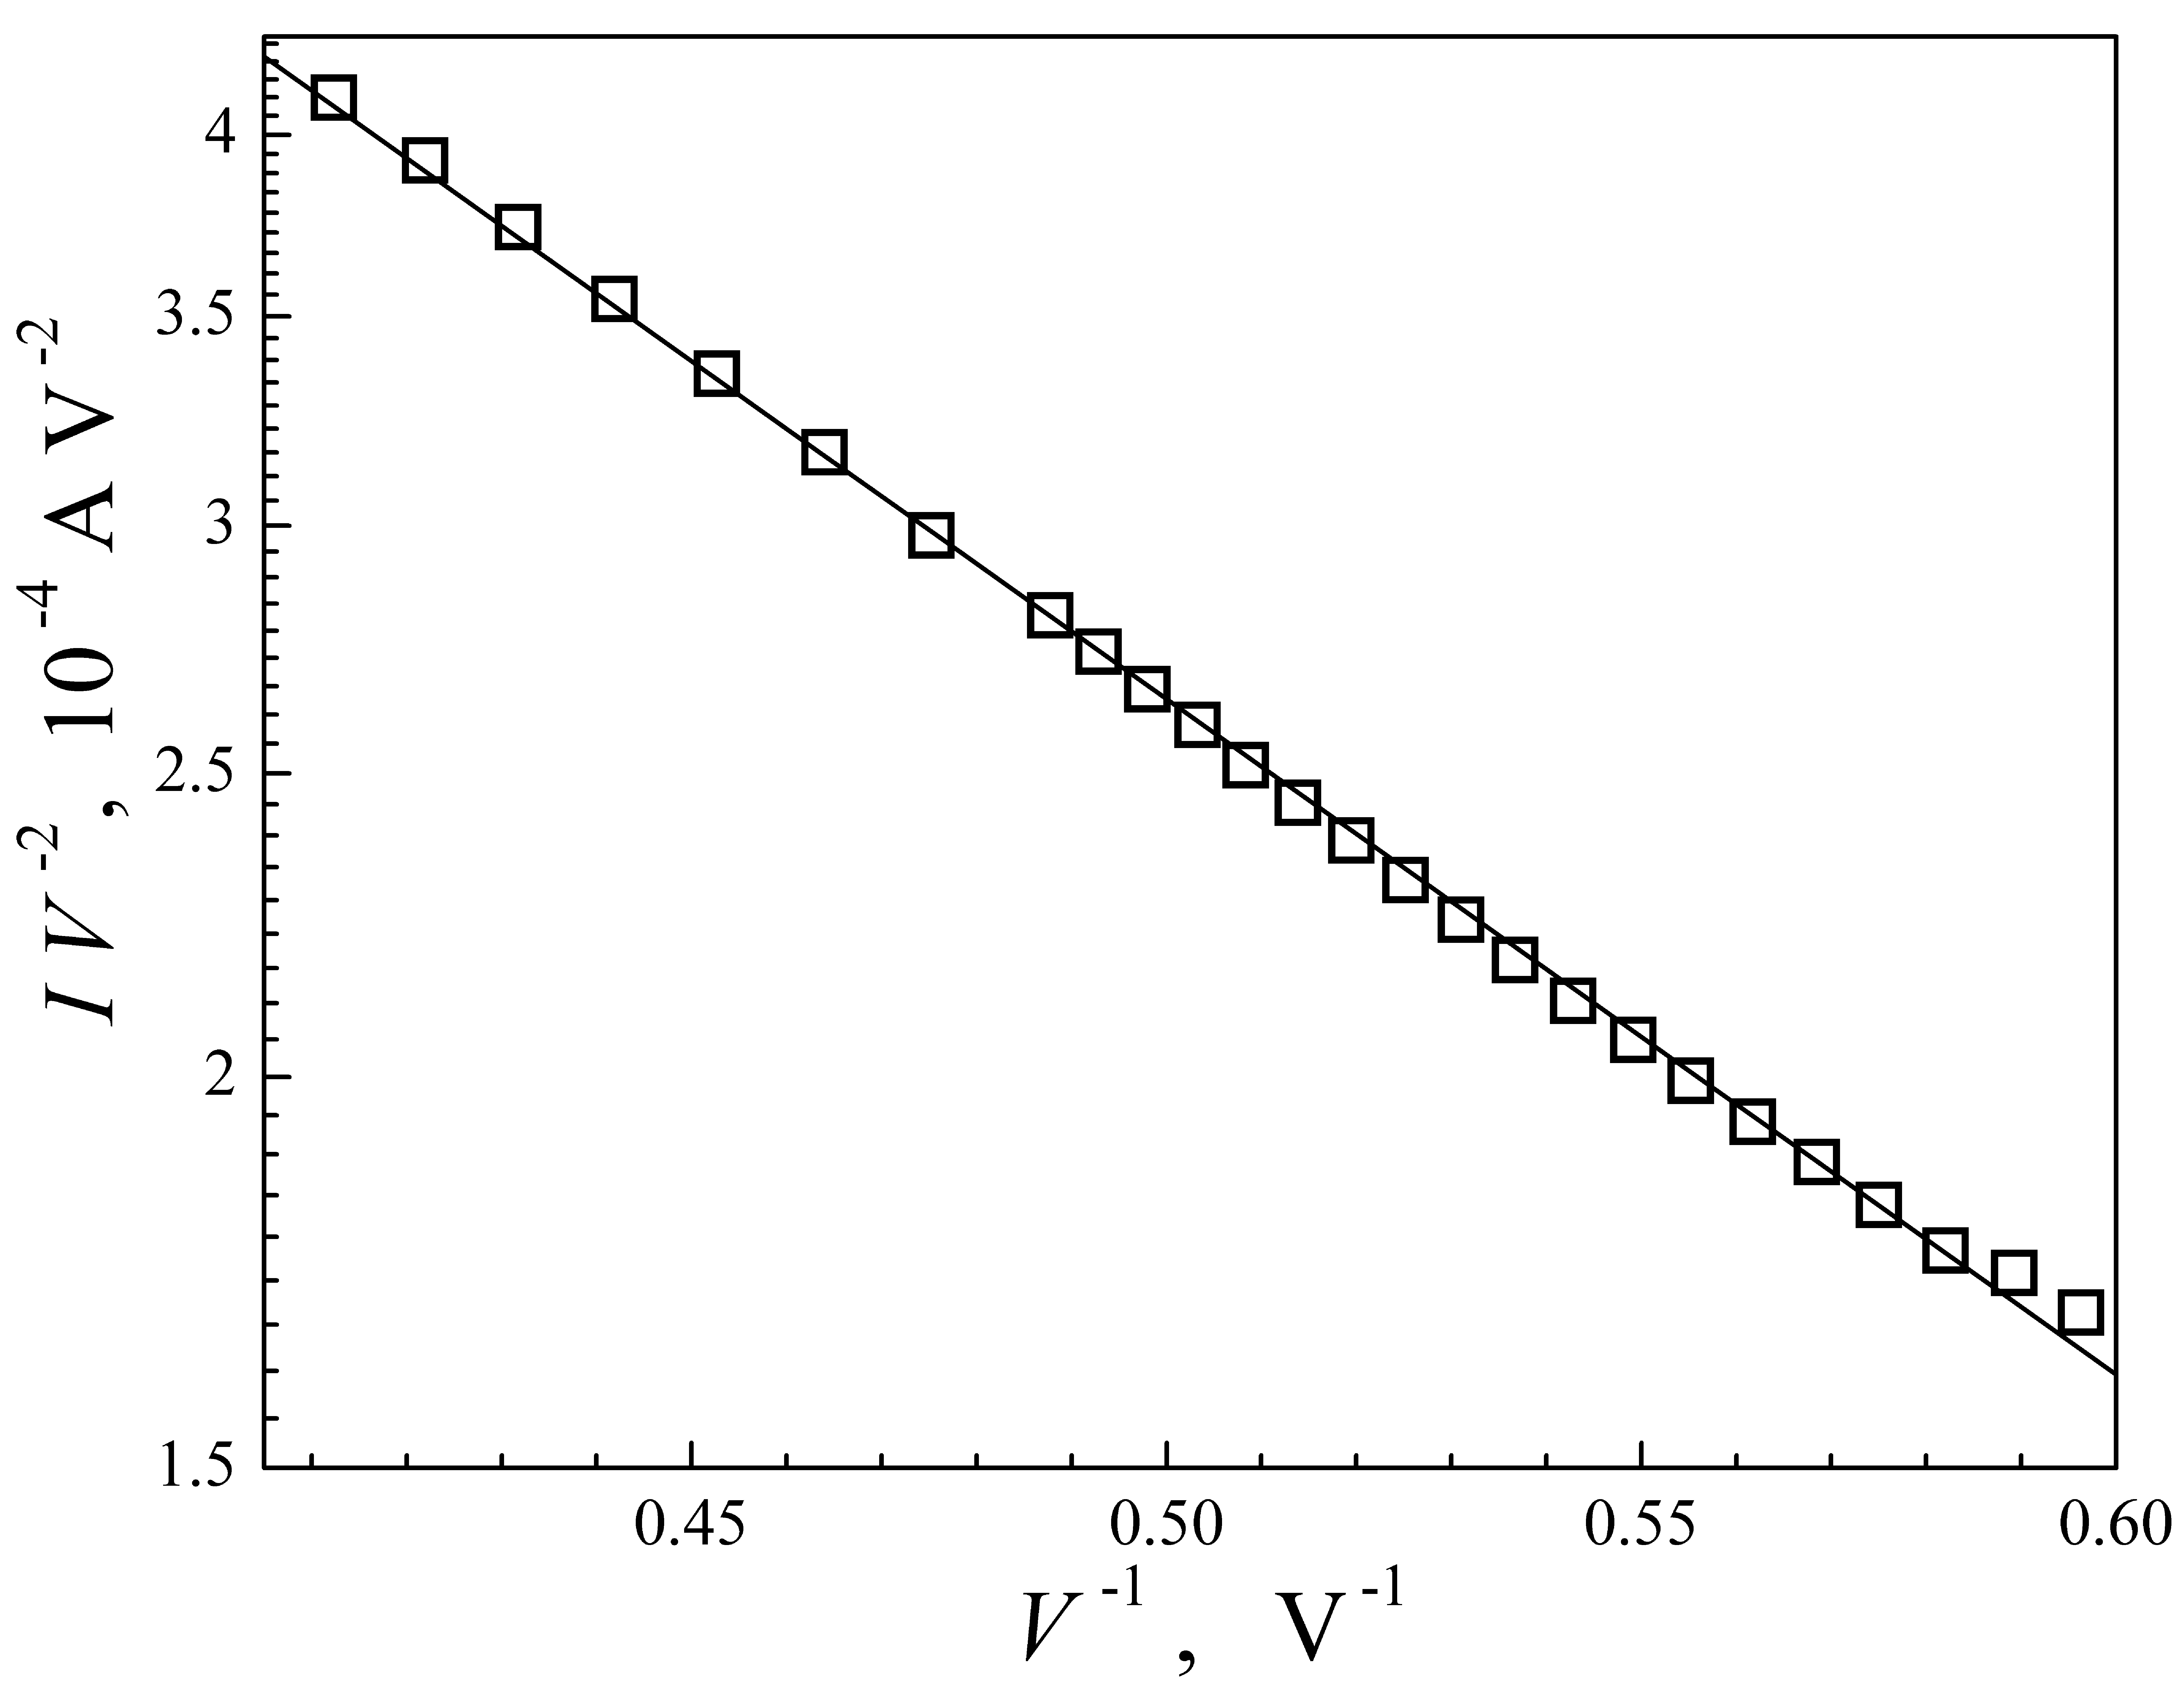
\includegraphics[width=0.6\textwidth]{FigFauler}}
\caption{\label{FigFauler}
The Fowler-Nordheim plot of the forward branch for non--irrradiated Au--SiO$_2$--Si structure at $V>1,6$~V.
The line is the least--squares linear fitting.
}%
\end{figure}

As shown in Fig.~\ref{figIV}, the $\gamma$--irradiation has a considerable effect on the current behavior.
The changes are pronounced for the reverse branch especially and the $I-V$ characteristic modification is the evidence of a transformation of the current transport mechanism.
Thus the forward $I-V$ dependence, expected according to TE model, is observed at $V>1$~V only  and the current value is much more then one in the non--irradiated case.
The fitting of the $V>1$~V region by Eq.~(\ref{eqSDIV}) shows that the irradiation leads to significant increase in both series resistance and ideality factor values --- see Table~\ref{tabMIS} data.
And the former significantly exceeds the resistance change, which has been observed in the bulk samples.
The ideality factor increase deals with the RDs formation  and results in the observed TE current decreasing.
Note that the effect of the radiation induced decreasing of MOS structure current is known
\cite{SiO2:Niu}.


Pintilie, \emph{et al}. \cite{FZSi:Rad} have investigated the RD formation by $^{60}$Co $\gamma$-radiation in silicon.
The both  growth method and resistivity have been analogous to structure under our investigation and the dose $9\cdot10^7$~rad has been used.
It has been shown that complexes VO$_i$, �$_i$C$_s$, $H$--centre (V$_2$O$_i$), $\Gamma$--centre, and interstitial defect $I^{0/-}$ are the main radiation defects.
The latest one is a secondary defect and its appearance leads to a conductivity compensation (inversion) \cite{FZSi:Rad}.

In our case the series resistance change in a range one order of magnitude above causes the reduction of voltage drop in the dielectric layer.
As a result, the electric field intensity was ceased to be sufficient for effective Fowler--Nordheim tunneling and the corresponding current component was not observed after irradiation.

Fig.~\ref{figIV}(d) shows that the forward $I-V$ characteristic of irradiated structures at low biases ($V<1$~V) is enough good described by a power law
\begin{equation}\label{eqVIsclc}
  I=I_0\,V^{\,m_\mathrm{F}},
\end{equation}
where
$m_\mathrm{F}=\frac{V}{I}\frac{\partial V}{\partial I}$ is the power--law parameter.
The relation (\ref{eqVIsclc}) is typical for the space charge limited current
(SCLC) \cite{SCLC:MA2016,Jafar,SCLC:Kaya} and the $m_\mathrm{F}$ value is connected with the energy distribution of traps, which emit carriers.
E.g. the value $m_\mathrm{F}\approx1,3$, which is observed for the investigated structure after $\gamma$--irradiation and before UST, is evident of the exponentially distributed traps.
It is known \cite{SCLC:MA2016,Jafar,SCLC:Kaya} that the $I_0$ depends on the total trap concentration $N_t$
\begin{equation}\label{eqIoSCLC}
  I_0\sim 1/N_t^{m_\mathrm{F}-1},
\end{equation}
and the temperature dependency of  power--law parameter is defined by equation
\begin{equation}\label{eqMT_IoSCLC}
  m_\mathrm{F}=1+T_c/T,
\end{equation}
where
$T_c$ is the characteristic temperature parameter of the trap distribution;
notably the trap concentration per unit energy range at an energy $E$ above the valence band
is proportional to $\exp(-E/kT_c)$.

The SCLC current�-voltage relation is often written as \cite{Jafar}
\begin{equation}\label{eqVIsclcT}
  I(V,T)=C\exp\left(-\frac{E_x}{kT}\right)\,V^{\,m_\mathrm{F}(T)},
\end{equation}
where
$C$ is the constant,
$E_x$ is the activation energy that defined by the level position of the filled traps to the conductivity band.
Fig.~\ref{figEa_MIS} shows the temperature dependence of the forward current.
Eq.~(\ref{eqMT_IoSCLC}) was taken into account when Fig.~\ref{figEa_MIS} plotting.
One can see that the experimental data are in good agreement with the fitting curve by Eq.~(\ref{eqVIsclcT}) for value $E_x=(0,32\pm0,01)$~eV.




\begin{figure}
\centerline{
\includegraphics[width=0.6\textwidth]{figEa_MIS}}
\caption{\label{figEa_MIS}
Temperature dependence of SCLC--current for $\gamma$--irrradiated Au--SiO$_2$--Si structure before UST at $V=0,4$~V.
The line is the least--squares linear fitting.
}%
\end{figure}

The $\gamma$--irradiation of Si--SiO$_2$ structures is known \cite{PersenkovBook} to lead to
a mechanical stress relaxation, a trap filling, and a new charged defect generation.
It is believed \cite{SiO2:Devine,SiO2:Lenahan} that the negative charge is trapped at the interface while the positive charge accumulates at $E'$--centers, $E'_\delta$--centers, and three strained bond  related centers.
However, the $E'$ and $E'_\delta$ concentration considerably overrides the bond  related centers concentration in the case of defect formation by  photons ($X$-- and $\gamma$--rays) \cite{SiO2:Devine}.
It should be noted that the low temperature as well as low partial oxygen pressure result in the thin SiO$_2$ layer formation in the structure under investigation.
But it is known \cite{SiO2:Cantin} that RDs, which appear in thin and thick layers, are the same.

Note that the hydrogen content is the key factor of a  generation of the electrically active RDs in silicon MOS structures \cite{SiO2:Cantin} and the SiO$_2$ layers, which are grown by thermal oxidation, are rich in an atomic hydrogen \cite{PersenkovBook}.
The irradiation is known \cite{SiO2:Mahapatra,SiO2:Esseni} to lead to the breaking of $\equiv\!\mathrm{Si}\!-\!\mathrm{H}$ bonds at the Si--SiO$_2$ interface and subsequent diffusion of released H species into the oxide bulk.
%The deep level formation is due to the breaking of interfacial $\equiv\!\mathrm{Si}\!-\!\mathrm{H}$ bonds under hot carriers present condition and subsequent diffusion of released H species into the oxide bulk \cite{SiO2:Mahapatra,SiO2:Esseni}.
The resulting unsaturated bonds $\equiv\mathrm{Si}-$ act as electronic traps.
Generally  such defects are distinguished by the orientation of the silicon substrate.
It is considered \cite{SiO2:Rev} that $P_b$ centers appear at (111)--oriented substrate interface whereas $P_{b1}$ and $P_ {b0}$ centers are typical in the case of (100)--oriented substrate.
Both $P_ {b0}$ and $P_{b1}$ are chemically identical to the $P_b$ center,
however the difference in an electrical activity is observed \cite{SiO2:Rev}.

The non--monotonic energy distribution of the interface levels is observed in  Si--SiO$_2$ structures, grown on $n$--type silicon crystal, after the $\gamma$--rays irradiation with dose above $5\cdot10^5$~rad \cite{PersenkovBook}.
According to Parchinskii, \emph{et al}. \cite{ParchSiO2}, the highest density of surface states is observed at $E_c-(0,32\pm0,04)$~eV.
This value coincides with the determined  $E_x$ value.
Therefore the current at low forward bias for irradiated structures deals with carriers, which are trapped  by $P_b$--centers.
Besides the negative charge accumulation at interface results in both barrier height increase and observed TE current decreasing.
But as mentioned above, the main reason of TE current reduction is the $n$ rise, which is induced  by RDs generation at silicon near surface region.

As shown in panel (b) and (d) of Fig.~\ref{figIV},
%Fig.~\ref{figIV},a and Fig.~\ref{figIV},d shown that
USTs cause an increase of  a space charge limited current.
In particular, SCLC exceeds the TE current at the whole used forward voltage interval in the
case of $t_\mathrm{UST}=60$~min.
We used Eq.~(\ref{eqVIsclc}) to fit experimental $I-V$ data of irradiated and ultrasonically treated structures.
The obtained fitting parameters are summarized in Table~\ref{tabMIS}.
According to Eq.~(\ref{eqIoSCLC}), the detected increase in $I_0$ value is evident of AI decrease in $P_b$--center concentration.
It was experimentally observed that the acousto-�defect interaction
in Si structures mainly cause atomic diffusion, transformation of native and impurity defects,
modification of interior surface states, and appearance of new defects \cite{Roman:2010JAP,Korotchenkov1995,Olikh2009Sem,UST:Medvid,OlikhJAP,Savkina2015}.
But the $P_b$--center annealing is known \cite{SiO2:Takakura,SiO2:Wurzer} to deal with the passivation of dangling bonds at the oxide--silicon interface by hydrogen atoms.
Thus the obtained results indicate about the AI diffusion of hydrogen.
Similar process has been reported  early \cite{Ostap:SiO2,Ostap:PhotoLum,ostapenko1997}, but the RDs acoustically--induced annealing was observed in our case.

The AI increase in $m_\mathrm{F}$ value (or $T_c$ rising --- see Eq.~(\ref{eqMT_IoSCLC})) testifies to the narrowing of the trap level energy distribution.
So it is known \cite{Jafar} that $m_\mathrm{F}=2$ is observed in the case of single--energy trap.
The detected narrowing of the energy distribution is evident of a AI passivation selectivity,
that is, UST leads to atomic hydrogen capture by dangling bonds, which correspond to certain levels only.
In our opinion, the key parameter of the bond ultrasound passivation is a mechanical stress, which are generally non--uniform at the interface.
The impurity diffusivity is known \cite{AZIZ2001} to depend on mechanical stress.
On the one hand, it can be a reason of a hydrogen displacement under acoustic loading condition.
On the other hand, the effectiveness of AI passivation is determined by a mechanical deformation level and UST  assists to the structure uniformity.

AI bond passivation lead to a decrease in interface negative charge, which is trapped by $P_b$--centers;
as a consequence,
a partial recovery of barrier height and a TE current increase  are observed --- see $I_s$ data in Table~~\ref{tabMIS}.
The detected decrease in the series resistance value after UST is evidence of the RDs annealing in the semiconductor bulk.

The hydrogen released during the irradiation  is potentially hazardous because of this  mobile  species  can  then \cite{SiO2:Devine,SiO2:DiMaria,SiO2:Mahapatra,SiO2:Esseni}
i)~interact with other bonded hydrogen at Si/SiO$_2$  interface  and give rise to additional $P_b$--centers;
ii)~move to semiconductor bulk and produce generation--recombination  sites  and boron  deactivation in  the Si  substrate;
iii)~migrate within the oxide and results in the creation of the bulk--oxide traps $E'$--centers, which is believed to be due to broken $\equiv\!\mathrm{Si}\!-\!\mathrm{O}$ bonds.
The $E'$---centre is a defect resulting from an oxygen vacancy in SiO$_2$ and traps positive charge \cite{SiO2:Takakura,SiO2:Devine}.
The  $E'$ total concentration is about $10^{18}$~cm$^{-3}$ in the case of $10^{7}$~rad $\gamma$--irradiation, but centers are non--uniformly distributed over oxide layer and
largest concentration are expected near Si/SiO$_2$  interface.
The broken $\equiv\!\mathrm{Si}\!-\!\mathrm{O}$ bonds are not known to recover at room temperature and the  $E'$ annealing temperature is equal (200$\div$400)$^\circ$C \cite{SiO2:Mahapatra}.

$E'$---centres at oxide bulk give rise to stress--induced leakage current (SILC)\cite{SiO2:Mahapatra,SiO2:DiMaria}.
It is precisely this current that is observed in the irradiated structure under reverse bias --- see panels (a) and (c) on  Fig.~\ref{figIV}.
In fact, the conduction mechanism responsible for SILC is generally assumed \cite{SiO2:Esseni,SiO2:DiMaria} to be a trap--assisted tunneling (TAT).
According to \cite{TAT:Gilmore,TAT:GopalSST,TAT:Gopal}, the field dependence of TAT current is described as
\begin{equation}\label{eqIVTAT}
  I_R=I_{0,\mathrm{TAT}}\,(U_d+V)\exp\left(-\frac{R_\mathrm{TAT}}{F_m}\right),
\end{equation}
where
$I_{0,\mathrm{TAT}}$ and $R_\mathrm{TAT}$ do not depend on voltage,
$I_{0,\mathrm{TAT}}$ is proportional to trap concentration,
$U_d$ is the barrier height.
The measured reverse $I-V$ branches were fitted by using Eq.~(\ref{eqIVTAT}).
It has been found that the experimental data are in good agreement with the fitting
curves (see Fig.~\ref{figIV}) for values, listed in Table~\ref{tabMIS}.
This confirms assumptions about the reverse current mechanism in the irradiated structures.
The current deviations at high bias probably caused by series resistance.

Table~\ref{tabMIS} data illustrate that USTs lead to decrease in $I_{0,\mathrm{TAT}}$ and barrier height values.
The former is evidence of low temperature (about~80$^\circ$C) AI annealing of radiation traps.
In our opinion, the $E'$--centers annealing is caused by acoustically stimulated diffusion of interstitial oxygen atoms.

UST of $\gamma$--irradiated  Au�-SiO$_2$�-Si structure leads to a forward current increase as well reverse current decrease.
Therefore the rectification factor $K_\mathrm{RECT}$, that has became considerably degraded after irradiation, was recovered by an acoustic wave action.
The $K_\mathrm{RECT}$ data at 0.5~V are listed in Table~\ref{tabMIS}.
Thereby in this work, it is demonstrated that it is possible to partially recovery the quality of $\gamma$--degraded silicon MOS structure by nearly room--temperature ultrasound treatment.

\section{Conclusion}
The experimental investigation of influence of $\gamma$--irradiation and ultrasound treatment on carrier transport in Au�-SiO$_2$�-Si structure has been carried out.
It has been shown that $\gamma$--irradiation gives rise the space charge limited current and the trap--assisted tunneling current at forward and reverse bias, respectively.
The investigation has revealed that ultrasound treatment leads to nearly room--temperature annealing of radiation defects ($P_b$--centers and $E'$---centres) and partially recovery of silicon MOS structure characteristics.
The acoustically induced annealing is caused  by the enhance of a diffusivity of interstitial species (hydrogen and oxygen) under ultrasound loading condition.
By relying  on increase in the value of power--law parameter of a space charge limited current,
it has been concluded that ultrasound treatment leads to narrowing of energy distribution of $\gamma$--induced traps at Si/SiO$_2$  interface.
Thus, ultrasound can be an effective tool for controlling metal�-semiconductor structure characteristics.

\bibliography{olikh}

\end{document}

